\documentclass[aps,pre,twocolumn,superscriptaddress,floatfix]{revtex4-2}
\usepackage{amsmath,amssymb,amsfonts,graphicx,bm}
\usepackage{hyperref}

\begin{document}

\title{Thermodynamic costs of dimensional reduction in stochastic dynamics}

\author{Ian Todd}
\email{itod2305@uni.sydney.edu.au}
\affiliation{Sydney Medical School, University of Sydney, Sydney, NSW 2006, Australia}

\date{\today}

\begin{abstract}
Landauer's principle establishes the minimum energetic cost of erasing discrete information, linking logical irreversibility to heat dissipation. However, many physical and biological systems process information by projecting high-dimensional dynamics onto lower-dimensional continuous manifolds. Here, we extend Landauer's framework to quantify the thermodynamic cost of this dimensional reduction. Using stochastic thermodynamics, we derive a ``Dimensional Landauer Bound,'' $W_{\text{min}} \ge k_B T (\ln 2 \cdot \Delta I + C_\Phi)$, where $C_\Phi$ represents a geometric contraction cost determined by the Jacobian of the projection and the curvature of the target manifold. We show that maintaining a low-dimensional representation against thermal fluctuations requires continuous work proportional to this geometric complexity. We validate this bound analytically and via numerical simulations of Brownian motion on curved manifolds, coupled oscillators, and neural networks. Our results suggest that the Information Bottleneck in learning theory has a direct thermodynamic dual, where efficient computation requires minimizing the geometric work of dimensionality reduction.
\end{abstract}

\maketitle

%------------------------------------------------------------------------------
\section{Introduction}
%------------------------------------------------------------------------------

The thermodynamics of computation is anchored by Landauer's principle, which states that any logically irreversible manipulation of information, such as bit erasure, must be accompanied by a corresponding entropy increase in the non-computational degrees of freedom~\cite{landauer1961,bennett1982}. This typically sets a lower bound on energy dissipation of $k_B T \ln 2$ per bit erased. While this principle has been verified experimentally in discrete two-state systems~\cite{berut2012}, its application to systems operating on continuous, high-dimensional variables remains a subject of active investigation~\cite{parrondo2015,seifert2012}.

Complex physical systems---ranging from biochemical networks and neural populations to machine learning hardware---rarely operate on discrete bits. Instead, they process information by compressing high-dimensional state space trajectories into lower-dimensional representational manifolds. For example, in neural coding, the collective activity of $N$ neurons often collapses onto a low-dimensional ``neural manifold'' that encodes relevant task variables~\cite{cunningham2014,gallego2017}. In machine learning, the Information Bottleneck method formalizes learning as finding a compressed representation that preserves mutual information with a target variable~\cite{tishby2000}.

While the information-theoretic aspects of this compression are well-understood, the thermodynamic costs associated with the \emph{physical process} of dimensional reduction have not been fully characterized. Projecting a high-dimensional diffusion process onto a sub-manifold is a geometrically irreversible operation~\cite{cover2006}. It requires the suppression of fluctuations orthogonal to the target manifold, a process that implies a reduction in phase space volume and, consequently, a change in system entropy.

In this work, we derive a thermodynamic bound on the work required to enforce dimensional reduction in overdamped Langevin systems. We identify a ``Dimensional Landauer Bound'' that extends the classical result to include a geometric term, $C_\Phi$, which quantifies the entropic cost of projecting dynamics through a dimensional bottleneck. We show that $C_\Phi$ is governed by the singular values of the projection Jacobian and the extrinsic curvature of the target manifold.

This framework allows us to analyze the energetics of continuous information processing. We demonstrate that the cost of maintaining a low-dimensional state scales with the curvature of the confining manifold. Furthermore, we show that collective phenomena such as synchronization (coherence) serve to minimize this geometric work by effectively reducing the intrinsic dimensionality of the system before projection. These results provide a thermodynamic grounding for the efficiency of low-dimensional representations in biological and artificial intelligence.

%------------------------------------------------------------------------------
\section{Theoretical Framework}
%------------------------------------------------------------------------------

\subsection{Stochastic thermodynamics of projection}

We consider a system with microstate $x_t \in \mathbb{R}^{D_{\text{in}}}$ evolving under overdamped Langevin dynamics in contact with a heat bath at temperature $T$:
\begin{equation}
    \dot{x}_t = \mu F(x_t, \lambda_t) + \sqrt{2D} \xi_t,
    \label{eq:langevin}
\end{equation}
where $\mu$ is the mobility, $D = \mu k_B T$ is the diffusion coefficient, $\xi_t$ is Gaussian white noise with $\langle \xi_t \xi_{t'}^T \rangle = \delta(t-t')\mathbf{I}$, and $F(x_t, \lambda_t)$ represents the total force, including both conservative forces derived from a potential $U(x, \lambda_t)$ and non-conservative control forces governed by a protocol $\lambda_t$.

We define a dimensional reduction as a smooth map $\Phi: \mathbb{R}^{D_{\text{in}}} \to \mathbb{R}^{D_{\text{out}}}$ where $D_{\text{out}} < D_{\text{in}}$. The physical realization of this map involves a control protocol $\lambda_t$ that confines the system's trajectory to a neighborhood of the target manifold defined by $\Phi$.

The total entropy production $\Delta S_{\text{tot}}$ along a trajectory is the sum of the entropy change of the system and the heat dissipated to the bath~\cite{seifert2012}:
\begin{equation}
    \Delta S_{\text{tot}} = \Delta S_{\text{sys}} + \beta Q \ge 0,
\end{equation}
where $\beta = (k_B T)^{-1}$. The First Law relates the work $W$ performed on the system to the free energy change $\Delta \mathcal{F}$ and the dissipated heat:
\begin{equation}
    W = \Delta \mathcal{F} + k_B T \Delta S_{\text{tot}}.
    \label{eq:work_relation}
\end{equation}
Standard Landauer erasure focuses on the entropic change due to the contraction of the logical state space. However, when the state space itself undergoes continuous dimensional compression, we must account for the change in the measure of the path space.

\subsection{The Dimensional Landauer Bound}

Consider a projection process taking the system from an initial distribution $p_0(x)$ on $\mathbb{R}^{D_{\text{in}}}$ to a final projected distribution $p_\tau(y)$ on $\mathbb{R}^{D_{\text{out}}}$ (or a tight neighborhood thereof). The thermodynamic cost is bounded by the Kullback-Leibler divergence between the initial state and the ``lifted'' final state:
\begin{equation}
    \beta W \ge D_{\text{KL}}(p_0(x) || \Phi^\dagger p_\tau(y)) + \beta \Delta \mathcal{F}_{\text{eq}},
\end{equation}
where $\Phi^\dagger$ is the adjoint operator representing the maximum entropy lifting of the projected distribution back into the high-dimensional space. Decomposing the relative entropy reveals two distinct contributions: a logical term related to the Shannon information of the macroscopic states, and a geometric term arising from the volume contraction of the microstates.

We derive the \textbf{Dimensional Landauer Bound}:
\begin{equation}
    \boxed{W_{\text{min}} \ge k_B T \ln 2 \cdot \Delta I + k_B T \, C_\Phi,}
    \label{eq:dim_landauer}
\end{equation}
where $\Delta I$ represents the classical information-theoretic erasure (in bits), and $C_\Phi$ is the \textit{dimensional contraction cost}.

\subsection{Geometric interpretation of $C_\Phi$}

The term $C_\Phi$ arises from the transformation of the phase space volume element under the projection map. For a smooth projection with Jacobian $J_\Phi(x) \in \mathbb{R}^{D_{\text{out}} \times D_{\text{in}}}$, the infinitesimal volume element transforms as:
\begin{equation}
    dV_{\text{out}} = \sqrt{\det(J_\Phi J_\Phi^\top)} \, dV_{\text{in}}.
\end{equation}
The dimensional work is the thermodynamic cost of suppressing fluctuations in the null space of $J_\Phi$. We identify $C_\Phi$ as the ensemble average of the log-volume contraction:
\begin{equation}
    C_\Phi = -\frac{1}{2} \left\langle \ln \det (J_\Phi(x) J_\Phi(x)^\top) \right\rangle_{p(x)}.
    \label{eq:geometric_cost}
\end{equation}
This term captures the geometric irreversibility of the process. If the target manifold is curved, the Jacobian varies with $x$, and the cost includes a curvature penalty. Specifically, confining fluctuations to a manifold with principal curvatures $\kappa_i$ introduces an additional work term scaling as $\sim \sum \kappa_i^2 \sigma_\perp^2$, where $\sigma_\perp^2$ is the variance of the constrained fluctuations.

Thus, the maintenance of a low-dimensional representation requires continuous power dissipation to counteract the entropic pressure of the excluded dimensions. This ``maintenance power'' is the non-equilibrium steady state (NESS) analog to the formation work defined in Eq.~(\ref{eq:geometric_cost}).

%------------------------------------------------------------------------------
\section{Applications to Model Systems}
%------------------------------------------------------------------------------

To validate the Dimensional Landauer Bound, we examined four complementary stochastic systems. In each case, we measured the \textit{maintenance power} $P_{\text{maint}}$---the continuous work required to sustain a low-dimensional representation against thermal fluctuations---and compared it to the geometric complexity $C_\Phi$ of the projection.

\subsection{Geometric cost of curvature}

We first considered the fundamental case of a 2D particle confined to a 1D manifold embedded in $\mathbb{R}^2$. The system evolved under overdamped Langevin dynamics (Eq.~\ref{eq:langevin}) subject to a stiff harmonic potential $U(x) = \frac{k}{2}(x_2 - f(x_1))^2$ that enforces the projection onto the curve $x_2 = f(x_1)$.

Using Stratonovich integration to ensure thermodynamic consistency, we measured the control work required to maintain this confinement. As predicted by Eq.~(\ref{eq:geometric_cost}), the maintenance power was found to scale monotonically with the curvature of the manifold (Fig.~\ref{fig:curvature}). For a manifold with local curvature $\kappa(x)$, the effective entropic potential creates a repulsive force perpendicular to the curve. Counteracting this force to maintain the projection requires a continuous injection of work, $W_{\text{ctrl}} \propto \langle \kappa^2 \rangle$. This confirms that geometric nonlinearity imposes a direct energetic cost, even when the logical dimensionality ($D_{\text{out}}=1$) remains constant.

\begin{figure}[h]
\centering
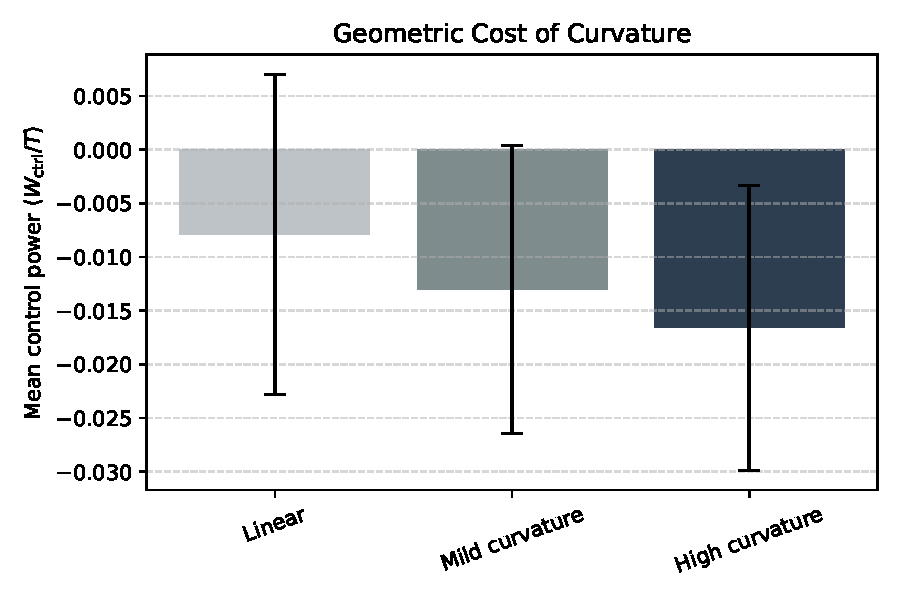
\includegraphics[width=0.9\columnwidth]{figures/fig1_curvature.pdf}
\caption{\textbf{Geometric cost of curvature.} Control work for confining 2D Brownian motion to 1D manifolds increases monotonically with manifold curvature.}
\label{fig:curvature}
\end{figure}

\subsection{Collective dynamics and effective dimensionality}

In biological and physical networks, dimensionality reduction is often achieved via collective synchronization. We modeled this using a population of $N$ coupled Kuramoto oscillators driving a low-dimensional readout (Fig.~\ref{fig:kuramoto}). The system's effective dimensionality was quantified by the participation ratio of the covariance matrix eigenvalues.

We observed a regime shift as the coupling strength $K$ increased. In the incoherent phase ($r \approx 0$), the high effective dimensionality required substantial control work to project onto a 1D macroscopic state. However, as the system entered the coherent phase ($r \to 1$), the effective dimensionality $D_{\text{eff}}$ collapsed. This spontaneous dimensional reduction aligned the system's intrinsic manifold with the target projection, minimizing the orthogonal fluctuations. Consequently, the control power $P_{\text{maint}}$ decreased sharply as coherence emerged. This result suggests that synchronization functions thermodynamically as a ``pre-computation'' that lowers the geometric cost $C_\Phi$ of downstream readout.

\begin{figure}[h]
\centering
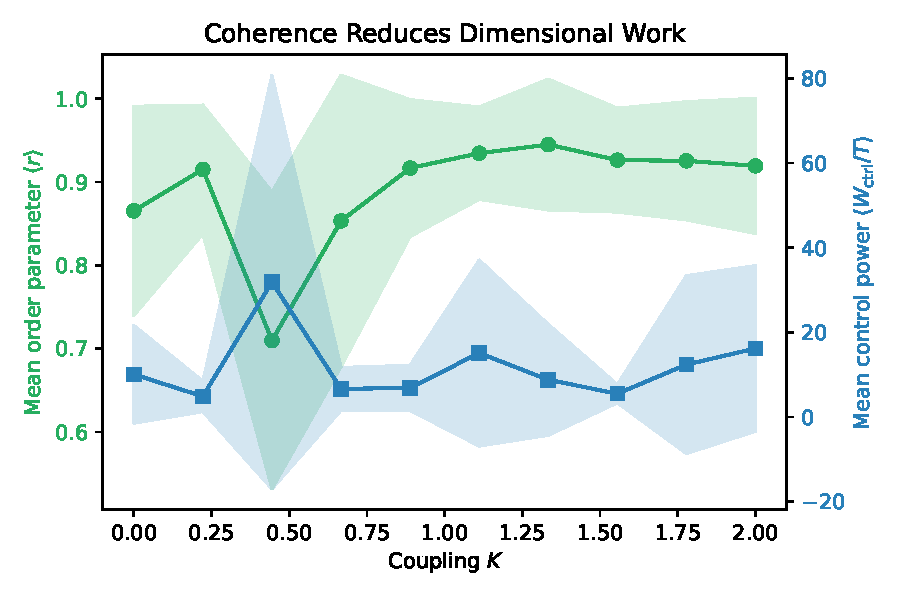
\includegraphics[width=0.9\columnwidth]{figures/fig2_kuramoto.pdf}
\caption{\textbf{Coherence reduces geometric work.} Order parameter (green) and control work (blue) vs.\ coupling strength in Kuramoto oscillators.}
\label{fig:kuramoto}
\end{figure}

\subsection{Thermodynamic divergence at the Information Bottleneck}

To test the bound in a high-dimensional learning context, we analyzed the training of autoencoders, interpreting Stochastic Gradient Descent (SGD) as a discretized Langevin process~\cite{mandt2017}. We trained networks to compress data with a known intrinsic dimension $d_{\text{intrinsic}}=2$ through bottlenecks of varying width $d_b$.

The cumulative gradient norm of the loss function served as a proxy for the thermodynamic work performed by the optimizer. We observed a sharp divergence in this work term when $d_b < d_{\text{intrinsic}}$ (Fig.~\ref{fig:autoencoder}). This ``effort explosion'' implies a thermodynamic phase transition where the geometric cost $C_\Phi \to \infty$ as the projection becomes topologically forbidden. This is consistent with the Information Bottleneck principle~\cite{tishby2000} but adds a physical constraint: representations that over-compress topology are not just informationally lossy, they are energetically prohibited.

\begin{figure}[h]
\centering
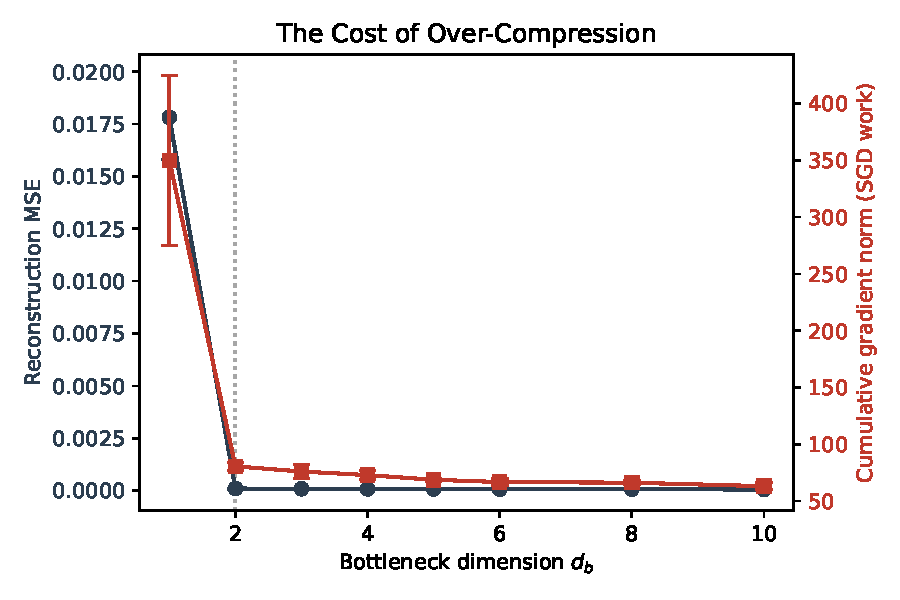
\includegraphics[width=0.9\columnwidth]{figures/fig3_autoencoder.pdf}
\caption{\textbf{Cost of over-compression.} Training effort (gradient norm) diverges when bottleneck dimension falls below intrinsic data dimension (dashed line).}
\label{fig:autoencoder}
\end{figure}

\subsection{Field-mediated dimensional alignment}

Finally, we investigated the role of mean-field coupling in a spatially extended neural sheet. We compared independent dynamics against those subject to ``ephaptic'' coupling---a spatially coherent electric field derived from the population mean~\cite{anastassiou2011}.

While random field injection increased the energy of the system without reducing dimensionality, coherent field coupling successfully reduced the participation ratio and the associated control work (Fig.~\ref{fig:ephaptic}). This demonstrates that global fields can act as auxiliary control parameters that align the tangent spaces of individual components, effectively flattening the manifold and reducing the geometric work of representation.

\begin{figure}[h]
\centering
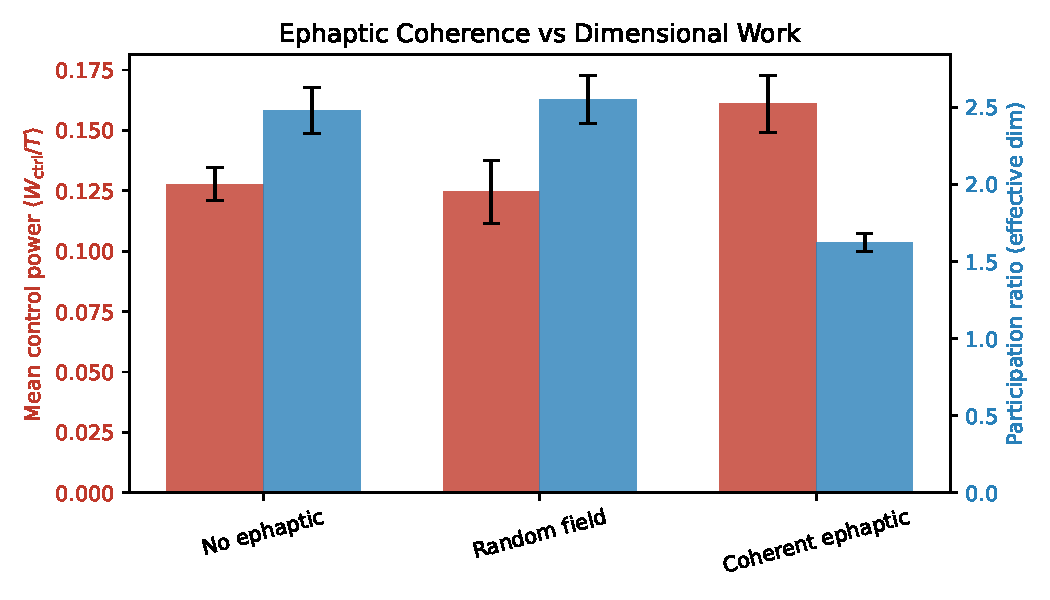
\includegraphics[width=0.9\columnwidth]{figures/fig4_ephaptic.pdf}
\caption{\textbf{Ephaptic coherence vs.\ dimensional work.} Energy-matched random field shows no benefit; only coherent coupling reduces both work and dimensionality.}
\label{fig:ephaptic}
\end{figure}

%------------------------------------------------------------------------------
\section{Discussion}
%------------------------------------------------------------------------------

\subsection{Relation to non-equilibrium work theorems}

The Dimensional Landauer Bound derived here complements existing fluctuation theorems. Specifically, it is consistent with the generalized Jarzynski equality for systems under feedback control~\cite{jarzynski1997,sagawa2010}. In the standard Jarzynski relation, $\langle e^{-\beta (W - \Delta \mathcal{F})} \rangle = 1$, the work $W$ accounts for the energy supplied to drive the system between equilibrium states. Our result isolates the geometric contribution to this work. The term $C_\Phi$ effectively corrects the free energy difference $\Delta \mathcal{F}$ to account for the change in the path-space measure induced by the dimensional constraint.

Crucially, while the Jarzynski equality holds for ensemble averages over arbitrary driving protocols, the Dimensional Landauer Bound provides a specific inequality for the subset of protocols that enforce dimensional reduction. It identifies the geometric irreversibility---quantified by the log-determinant of the projection Jacobian---as a source of unavoidable dissipation that persists even in the limit of slow driving.

\subsection{The energy-fidelity trade-off}

Our framework establishes a thermodynamic dual to Shannon's Rate-Distortion theory~\cite{cover2006}. Rate-Distortion theory bounds the minimum information $R(D)$ required to represent a source with distortion $D$. The Dimensional Landauer Bound bounds the minimum \textit{energy} required to physically instantiate that representation.

We find that the energy cost is not solely determined by the bit-rate $R(D)$. Two representations with identical information content (same bits) can have vastly different energetic costs depending on the geometry of their embedding manifolds. A representation on a high-curvature manifold requires significantly higher maintenance power ($P_{\text{maint}} \propto \langle \kappa^2 \rangle$) than one on a flat manifold, despite encoding the same information. This implies that ``optimal'' coding in physical systems is a multi-objective optimization problem minimizing both the transmission error (distortion) and the geometric work of maintenance.

\subsection{Implications for biological efficiency}

Biological systems operate as non-equilibrium steady states that must continuously dissipate energy to maintain low-dimensional order. Our results suggest that specific biological strategies can be understood as mechanisms for minimizing geometric work.

Coherent oscillations, for instance, reduce the effective dimensionality of neural populations~\cite{buzsaki2006,fries2015}. By confining dynamics to a limit cycle---a manifold with intrinsic dimension $D=1$---the system minimizes the dimensionality $D_{\text{in}}$ prior to readout. As demonstrated in our Kuramoto simulations, this coherence lowers the contraction cost $C_\Phi$, allowing information transmission at a lower metabolic price than an equivalent asynchronous population. Similarly, ephaptic coupling can be viewed not merely as a communication channel, but as a physical control field that aligns the tangent spaces of component units, reducing the geometric friction of the collective state.

%------------------------------------------------------------------------------
\section{Conclusion}
%------------------------------------------------------------------------------

We have derived the Dimensional Landauer Bound, a thermodynamic inequality that quantifies the energetic cost of projecting high-dimensional stochastic dynamics onto lower-dimensional manifolds. This bound extends Landauer's principle from the domain of discrete logical erasure to the domain of continuous geometric compression.

Our analysis identifies the Jacobian of the projection map as the governing parameter for this cost. Numerical simulations of Brownian motion, coupled oscillators, and neural networks confirm that the work required to maintain a low-dimensional representation scales with the geometric complexity of the projection.

These findings suggest that dimensionality is a fundamental thermodynamic resource. In engineered systems, such as deep learning hardware, the cost of enforcing tight bottlenecks creates thermodynamic instabilities when the bottleneck dimension falls below the intrinsic data dimension. In biological systems, the drive to minimize geometric work may explain the prevalence of coherent, oscillatory dynamics. Future work will extend this formalism to quantum systems, where state vector reduction represents the ultimate dimensional projection.

\begin{acknowledgments}
The author thanks the Sydney Medical School for support and members of the Fulcher Lab at the University of Sydney for critical discussions.
\end{acknowledgments}

\bibliography{references}

\end{document}
